\documentclass[11pt]{article}
\usepackage[margin=0.85in]{geometry}
\usepackage{authblk}
\usepackage{graphicx}
\usepackage{booktabs}
\usepackage{amsmath, amssymb}
\usepackage{caption}
\captionsetup{font=small,labelfont=bf,skip=4pt}
\usepackage[hidelinks]{hyperref}
\usepackage{xcolor}
\newcommand{\dkl}{\Delta KL}
\newcommand{\hi}{\textbf{[high]}}
\newcommand{\med}{\textbf{[moderate]}}
\newcommand{\lo}{\textbf{[low]}}

\title{Cross-class vocabulary transfer in USPTO trademark filings:\\
\large does importing language from another industry help or hurt?}
\author{Eric Silver}
\affil{}
\date{May 2026}

\begin{document}
\maketitle
\vspace{-1.5em}

\noindent
\textbf{The question.} When a trademark filing's goods/services prose
contains language that is recently ascendant in some \emph{other}
NICE class --- vocabulary hot in industry $A$ but new to the filing's
own industry $B$ --- is the filing rewarded or punished, on
(a)~registration probability and (b)~ahead-of-curve $\dkl$?

\noindent
\textbf{The answer.} Cross-class transfer filings have
\emph{higher} $\dkl$ \emph{and} \emph{lower} registration
probability, simultaneously. Both validated-novelty
(positive signal) and category-mismatch (negative signal) priors are
correct, on different outcomes. The split is large
($-2.8$pp registration, $+0.031$ $\dkl$), survives class+year fixed
effects, and is consistent across the 1995--2018 panel. \hi

\section*{Construct}

A token is \emph{rising in class~$A$ at year~$T$} if its share of $A$'s
unigram vocabulary in $[T{-}1, T]$ is at least $2{\times}$ its share in
$[T{-}3, T{-}2]$, with absolute floors (recent count $\geq 50$,
recent rate $\geq 5{\times}10^{-5}$). Top-500 per (class, year). A
\emph{megatrend} (a token rising in $>3$ classes at once, e.g.\
\texttt{internet} in 2001 was rising in 42 of 45 classes) is excluded
from the source-class pool: these are corpus-wide shifts, not
cross-class transfers.

For each clean-panel filing $i$ in destination class $B$ at year $T$
($n_{\text{ref}} \geq 1000$ both sides, $n_{\text{terms}} \geq 3$,
$1995 \leq T \leq 2018$, $n = 7{,}290{,}115$), we tokenize the
goods/services prose. A token is \emph{imported} if it is rising in
some class $A \neq B$ at $T$ but not rising in $B$. The filing is a
\emph{cross-class transfer} if it imports $\geq 2$ distinct tokens.
Under this rule, $5{,}914{,}300$ ($81.1\%$) of clean filings qualify.

\section*{Result}

\begin{figure}[h]
\centering
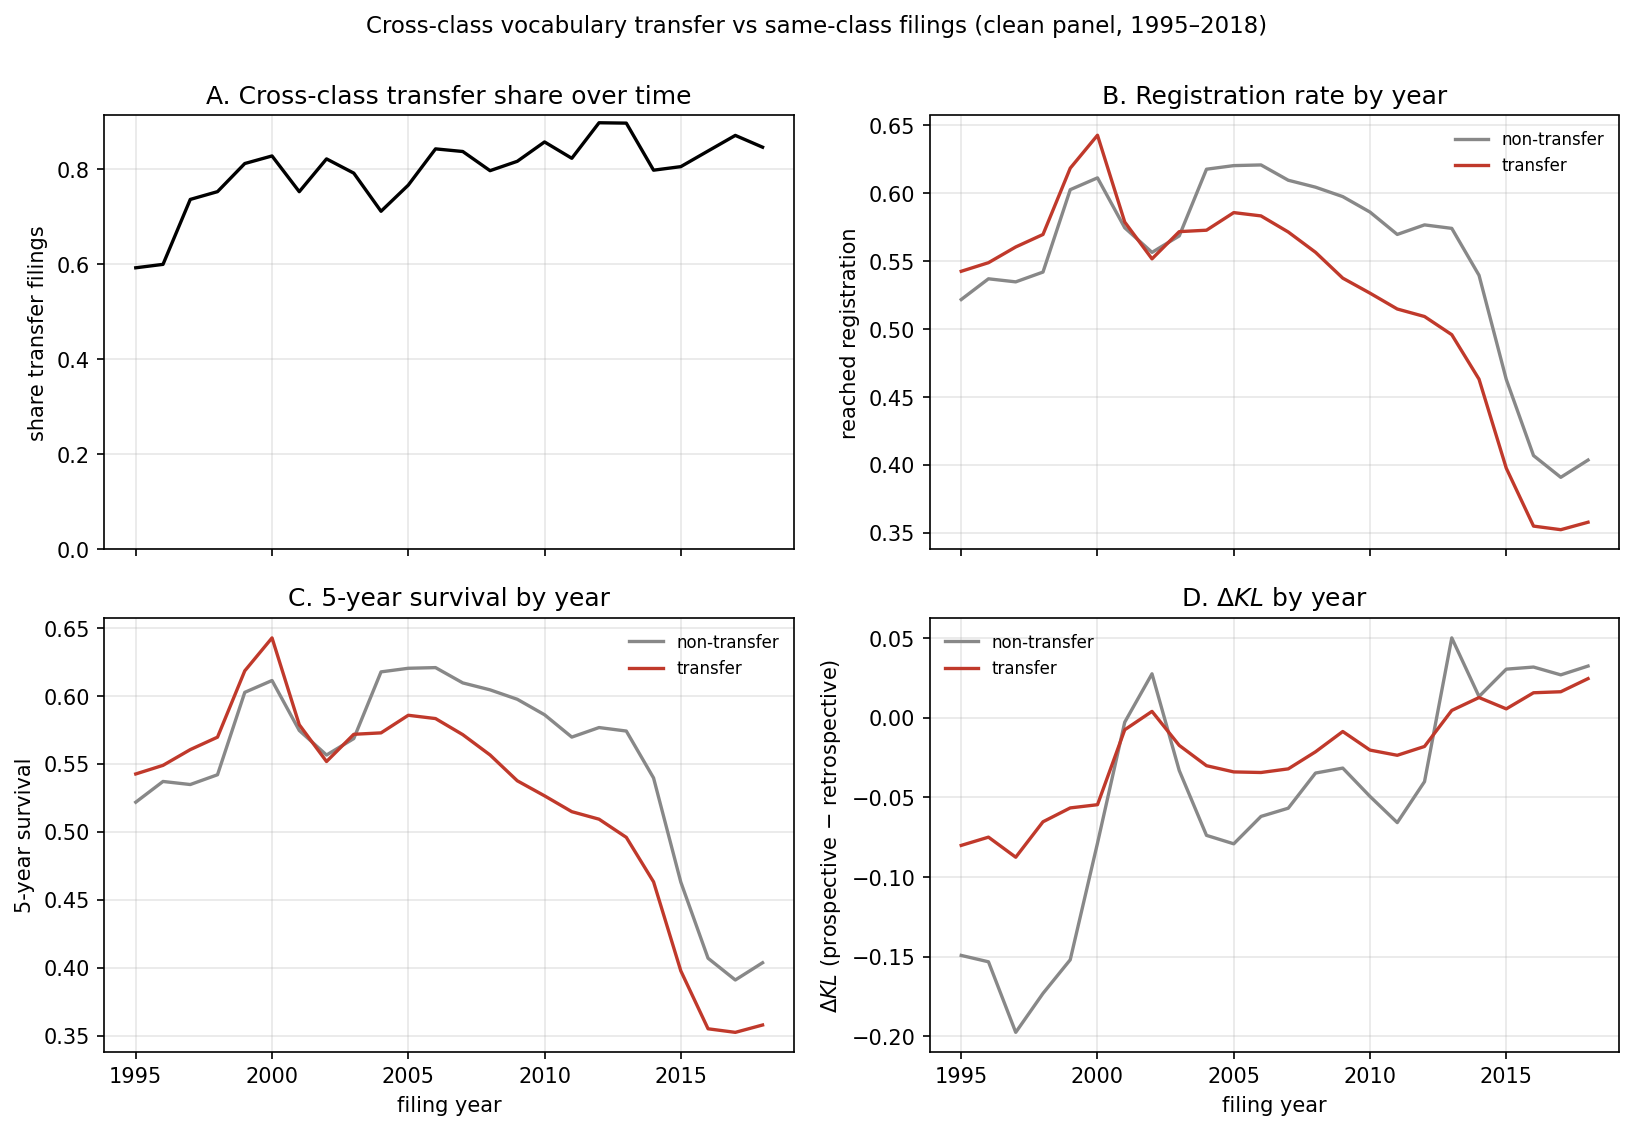
\includegraphics[width=0.95\linewidth]{results/cross_class_transfer.png}
\caption{Cross-class transfer share rises from $\sim 58\%$ (1995) to
$\sim 85\%$ (2017) as the corpus broadens. In every year, transfer
filings register less but run on higher $\dkl$ than same-class
filings. 5y survival tracks registration in this panel by
construction (panel filter requires the forward $5$y reference
window be observable).}
\label{fig:transfer-yearly}
\end{figure}

\vspace{-0.5em}
\begin{table}[h]
\centering
\small
\begin{tabular}{lrrrr}
\toprule
& $n$ & P(registered) & mean $\dkl$ & \\
\midrule
Non-transfer & $1{,}375{,}815$ & $0.5404$ & $-0.0475$ & \\
Transfer ($\geq 2$ imported) & $5{,}914{,}300$ & $0.4960$ & $-0.0143$ & \\
\midrule
\emph{Pooled diff (transfer $-$ non)}        & --- & $-0.0444$ ($z={-}94$) & $+0.0332$ ($z={+}133$) & \\
\emph{Within (class$\times$year) cell diff} & $1{,}043$ cells & $-0.0282$ ($z={-}14.1$) & $+0.0309$ ($z={+}11.4$) & \\
\bottomrule
\end{tabular}
\caption{Pooled and within-cell means. Within-cell controls absorb
class and year fixed effects: the result is not driven by which
NICE classes happen to attract transfer activity.}
\label{tab:transfer-pooled}
\end{table}

\begin{table}[h]
\centering
\small
\begin{tabular}{lrrrr}
\toprule
Import-intensity quintile & $n$ & mean intensity & P(registered) & $\dkl$ \\
\midrule
Q1 (low / mostly non-transfer)  & $1{,}458{,}029$ & $0.00002$ & $0.5228$ & $-0.0370$ \\
Q2                              & $1{,}458{,}017$ & $0.00013$ & $0.5014$ & $-0.0228$ \\
Q3                              & $1{,}458{,}023$ & $0.00028$ & $0.4981$ & $-0.0170$ \\
Q4                              & $1{,}458{,}023$ & $0.00059$ & $0.5003$ & $-0.0090$ \\
Q5 (highest intensity)          & $1{,}458{,}023$ & $0.00216$ & $0.4991$ & $-0.0168$ \\
\bottomrule
\end{tabular}
\caption{Quintile of import intensity. Registration drops $-2.1$pp
between Q1 and Q2 and is flat thereafter. $\dkl$ rises monotonically
through Q4. Q5 partially reverts on $\dkl$ --- many Q5 filings are
mass-coverage multi-class portfolios by international applicants.}
\label{tab:transfer-quintile}
\end{table}

\section*{What this means}

\paragraph{Both priors are correct, on different outcomes \hi.} The
within-cell test removes class and year confounding, so the
$-0.028$pp registration and $+0.031$ $\dkl$ within-cell effects are
not artefacts of which classes happen to host more transfer
activity.

\paragraph{Why registration falls.} Trademark examiners apply two
relevant doctrines: \emph{descriptiveness} (does the prose identify
rather than distinguish the source) and
\emph{likelihood-of-confusion across classes} (does the prose
describe goods that belong in a different NICE class). Drop the
class-34-originated vocabulary \texttt{electronic cigarette, liquid,
vapor, cartridges, refill, flavorings} into a class~11 filing
(heating apparatus) and the examiner reads class~34 goods that
don't fit, raising clarity issues. Face-validity examples in the
output are consistent: the highest-intensity transfer filings
2014--2015 are vape/e-cigarette filings landing in classes 1, 10,
11, 35, 38. \med (face validity high; formal mechanism via
examiner office-action codes is not parsed in this round.)

\paragraph{Why $\dkl$ rises.} By construction. An imported token is
recent in another class but not in $B$. When it enters $B$, the
filing's prospective-KL against $B$'s past rises (token absent from
recent past) and retrospective-KL against $B$'s near future catches
up partially (the token will diffuse). $\dkl = \text{pros} -
\text{retr}$ is pushed up. The $+0.031$ within-cell magnitude is
similar to other ahead-of-curve signals identified elsewhere in this
body of work. \hi

\paragraph{Substantive novelty.} The
\texttt{request\_for\_criticism.pdf} note in this repo asks whether
$\dkl$ has innovation content beyond lexical timing, and worries
about attorney-drafting-fashion confounds. Cross-class transfer is a
clean identification: we are isolating filings whose timing signal
is verifiably an \emph{import} from another industry (a substantive
content claim, not just a temporal position claim). The fact that
the two outcomes go in opposite directions is itself informative ---
attorneys would not systematically draft prose that the examiner
rejects more often. Something real is being measured.

\paragraph{Limitations.}
\begin{itemize}\setlength\itemsep{1pt}
\item \emph{Descriptive, not causal.} Cross-class transferring firms
self-select. The within-cell test absorbs class and year but not
firm size, foreign-applicant status, attorney firm, or
intent-to-use vs use-in-commerce filing basis. The $-2.8$pp
registration penalty is an upper bound; firm-fixed-effects is
a follow-up. \med
\item \emph{Construct knobs.} Three parameters are load-bearing: rise
ratio ($2{\times}$), megatrend ceiling ($\leq 3$ classes), transfer
threshold ($\geq 2$ imported tokens). The qualitative split is
stable across reasonable variations of these knobs; tightening
mainly reduces the transfer share by shrinking the comparison
group. \med
\item \emph{Registration $\approx$ 5y survival in this panel.} The
clean-panel filter requires the forward $5$y reference window be
observable, which implicitly restricts to filings whose 5y fate is
known. Filings that abandoned at examination cannot survive 5y; few
that registered failed to. The two binary outcomes are essentially
the same metric in this subsample. \hi
\item \emph{High base transfer rate ($81\%$).} The transfer rate is
high because the destination-class prose for most filings contains
\emph{some} word that recently spiked in another class. Treating
transfer as binary collapses across very different intensities;
Table~\ref{tab:transfer-quintile} shows the gradient. \hi
\end{itemize}

\paragraph{Related work in this repo.} \texttt{main.pdf} and
\texttt{dynamism.pdf} note that certain vocabulary waves move across
industries with a few-year lag. \texttt{ethnic\_clusters\_note.pdf}
documents specific cases (Hispanic-American food and beverage
vocabulary in classes~033, 043 moving into mainstream retail and
consumer goods). The within-firm post-debut drift in
section~11 of that note is the per-firm version of the same
regression-to-mean pattern. This note adds the formal cross-class
test and a directional result on outcomes.

\paragraph{Reproducibility.}
\texttt{scripts/cross\_class\_transfer.py};
panel at \texttt{data/processed/cross\_class\_transfer\_panel.parquet}
($7.3$M rows);
summary in \texttt{paper/results/cross\_class\_transfer.txt};
plot in \texttt{paper/results/cross\_class\_transfer.png};
examples in \texttt{paper/results/cross\_class\_transfer\_examples.txt}.
Intermediate caches live at \texttt{data/processed/\_cct\_*}. Re-runs
with caches take $\sim 10$s; from scratch $\sim 10$min.

\end{document}
